\documentclass{article}
\usepackage{CJKutf8}
\usepackage{graphicx}
\usepackage{enumerate}
\usepackage{amsmath}
\usepackage{amsthm}
\usepackage{amsfonts}
\usepackage{hyperref}
\usepackage{subfigure}
\usepackage{amsmath}

\usepackage{algorithm}
\usepackage{algpseudocode}
\usepackage{amsmath}
\renewcommand{\algorithmicrequire}{\textbf{Input:}}  % Use Input in the format of Algorithm
\renewcommand{\algorithmicensure}{\textbf{Output:}} % Use Output in the format of Algorithm
\usepackage{listings}
\usepackage{url}

\usepackage{etoolbox}
\newtoggle{solution}
% \toggletrue{solution}
\togglefalse{solution}

\usepackage{color}
\usepackage[dvipsnames]{xcolor}
\newcommand{\solution}[2][0pt]{\iftoggle{solution}{\smallskip{\color{red}{\flushleft\textbf{Solution}:}\par#2}}{\vspace*{#1}}}

\renewcommand{\baselinestretch}{1.2}%Adjust Line Spacing
%\geometry{left=2.0cm,right=2.0cm,top=2.0cm,bottom=2.0cm}% Adjust Margins of the File

% Create horizontal rule command with an argument of height
\newcommand{\horrule}[1]{\rule{\linewidth}{#1}}
% Set the title here
\title{
    \normalfont \normalsize
    \textsc{ShanghaiTech University} \\ [25pt]
    \horrule{0.5pt} \\[0.4cm] % Thin top horizontal rule
    \huge CS240 Algorithm Design and Analysis \\ % The assignment title
    \LARGE Spring 2024\\
    \LARGE Problem Set 5\\
    \horrule{2pt} \\[0.5cm] % Thick bottom horizontal rule
}
% wrong usage of \author, never mind
\author{Name: Zhou Shouchen\\\\StudentID: 2021533042\\\\}

\date{Due: 11:59pm, June 14, 2024}

% Add the support for auto numbering
% use \problem{title} or \problem[number]{title} to add a new problem
% also \subproblem is supported, just use it like \subsection
\newcounter{ProblemCounter}
\newcounter{oldvalue}
\newcommand{\problem}[2][-1]{
	\setcounter{oldvalue}{\value{secnumdepth}}
	\setcounter{secnumdepth}{0}
	\ifnum#1>0
		\setcounter{ProblemCounter}{#1}
	\else
		\stepcounter{ProblemCounter}
	\fi
	\section{Problem \arabic{ProblemCounter}: #2}
	\setcounter{secnumdepth}{\value{oldvalue}}
}
\newcommand{\subproblem}[1]{
	\setcounter{oldvalue}{\value{section}}
	\setcounter{section}{\value{ProblemCounter}}
	\subsection{#1}
	\setcounter{section}{\value{oldvalue}}
}

\begin{document}
\maketitle
\vspace{3ex}

\begin{enumerate}
%\item Please write your solutions in English
\item Submit your solutions to the course Gradescope.
\item If you want to submit a handwritten version, scan it clearly.
%\item Late homeworks submitted within 24 hours of the due date will be marked down 25\%.  Homeworks submitted more than 24 hours after the due date will not be accepted unless there is a valid reason, such as a medical or family emergency.
\item You are required to follow ShanghaiTech's academic honesty policies.  You are allowed to discuss problems with other students, but you must write up your solutions by yourselves.  You are not allowed to copy materials from other students or from online or published resources.  Violating academic honesty can result in serious penalties.
\end{enumerate}

\newpage

\problem{}

Given a set $C$, a collection of subsets of $C$ and an integer $k \geq 1$, the Set-Packing problem asks if there are $k$ subsets from the collection which are pairwise disjoint (i.e. no two sets share an element). Show that the Set-Packing problem is NP-complete.

\solution{}






\newpage
\problem{}

Given a Boolean CNF (conjunctive normal form) formula $\phi$ and an integer $k \geq 1$, the Stingy-SAT problem asks whether the formula has a satisfying assignment in which at most $k$ variables are set to true. Prove that Stingy-SAT is NP-complete.

\solution{}

1. Stingy-SAT is in NP.\\
We can varify a CNF formula \(\phi\) is satisfied or not in polynomial time.\\
And then check the number of variables set to true is no more than \(k\) in $O(n)$ time, where $n$ is the length of $\phi$.\\
So the total time complexity is polynomial.\\
So Stingy-SAT $\in$ NP.\\

2. SAT $\leq_p$ Stingy-SAT.\\
We can reduce SAT to Stingy-SAT.\\
Given a SAT problem, we additionally check whether the number of variables set to true is no more than \(k\).\\

<1> "$\Rightarrow$":\\
If the SAT problem with firmula $\phi$ with $k$ variables is satisfied, then the number of variables set to true is no more than \(k\).\\
So the Stingy-SAT $(\phi,k)$ is satisfied.\\

<2> "$\Leftarrow$":\\
If the Stingy-SAT $(\phi,k)$ is satisfied, then without the constrains of $k$, the SAT problem is also satisfied.\\

<3> Polynomial Time:\\
The construction only needs to check the number of variables set to true, which is in $O(n)$ time.\\
So it could be done in polynomial time.\\
So we have proved that SAT $\leq_p$ Stingy-SAT.\\

Since SAT $\in$ NP-complete; Stingy-SAT$\in$ NP; SAT $\leq_p$ Stingy-SAT.\\
Therefore, Stingy-SAT $\in$ NP-complete.\\

So above all, we have proved that Stingy-SAT is a NP-complete problem.

\newpage
\problem{}
A thief is planning to rob houses along a street. Each house has a certain amount of money stashed, and the thief can rob any set of houses, as long as he does not rob any adjacent houses.  Determine the maximum amount of money the thief can steal.

\solution{}



For loop in the pseudo-code is form `$\textbf{for } i \gets 1 \textbf{ to } n$' represents $i=1,2,\cdots,n$ sequentially.
\begin{algorithm}
    \caption{Maximum stolen money}\label{alg:problem-3}
    \begin{algorithmic}[1]
    \State \textbf{Input:} Number of house $n$, each house's money number $a_1, a_2, \cdots, a_n$. 
    \State \textbf{Output:} The maximum number of money could steal $ans$.
    \State $dp(1,0) \gets 0, dp(1,1)\gets a_1$
    \For{$i \gets 2$ \textbf{to} $n$}
        \State $dp(i,0) \gets \max\{dp(i-1,0),dp(i-1,1)\}$
        \State $dp(i,0) \gets dp(i-1,0)+a_i$
    \EndFor
    \State $ans \gets \max\{dp(n,0),dp(n,1)\}$
    \State \textbf{return} $ans$
    \end{algorithmic}
\end{algorithm}





\newpage
\problem{}
Consider an $n \times n$ grid graph $G$, as shown below.

\begin{figure}[h]
    \centering
    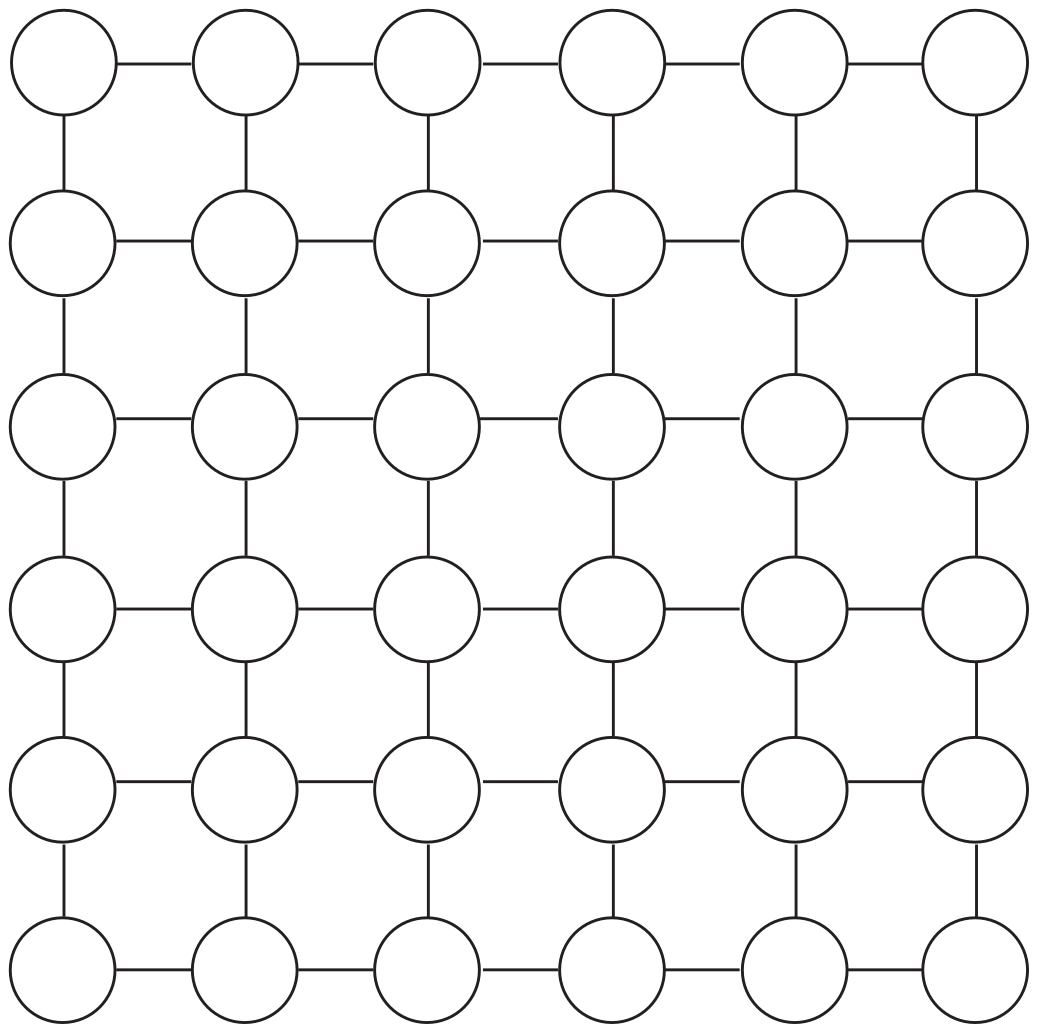
\includegraphics[width=0.4\linewidth]{media/p4.png}
\end{figure}

Each node $v$ in $G$ has a weight $w(v) > 0$.  You want to choose an independent set of nodes with maximum total weight.  That is, you want to choose a set of nodes $S$ with maximum total weight such that for any $v \in S$, none of $v$'s neighbors are in $S$.  To do this, consider the following greedy algorithm.  Let $V$ be the set of all nodes in $G$.  Choose the node in $V$ with the largest weight (breaking ties arbitrarily), add it to the independent set, then remove the node and all its neighbors from $V$.  Repeat this process until $V$ is empty.  Let $S$ be the output of this algorithm.   Solve the following problems.

\begin{enumerate}
\item Let $T$ be any independent set in $G$.  Show that for each node $v \in T$, either $v \in S$, or there is a neighbor $v'$ of $v$ with $v' \in S$ and $w(v) \leq w(v')$.
\item Show that the greedy algorithm is a 4-approximation.
\end{enumerate}

\solution{}
1. <1> If $v \in S$, then according to the definition of the independent set, we could get that for any neighbor    $v'$ of $v$, $v' \notin S$.

<2> If $v \notin S$, then according to the independent set, there exist at least one neighbor $v'$ of $v$ such that $v' \in S$. \\
And according to the greedy algorithm, we could get if for all neighbors $v'$ of $v$, $v'\in S$ has that $w(v')<w(v)$, the algorithm would choose $v$ before $v'$, which contradicts the greedy algorithm. So there must exist a neighbor $v'$ of $v$ such that $v' \in S$ and $w(v) \leq w(v')$.

So above all, we have proved that for each node $v \in T$, either $v \in S$, or there is a neighbor $v'$ of $v$ with $v' \in S$ and $w(v) \leq w(v')$.\\

2. Suppose that the greedy algorithm chooses the nodes consisting of $S$, and the optimal solution chooses the nodes consisting of $S^*$.\\

According to 1, we could get that for each node $v \in S$, either $v \in S^*$, or there is a neighbor $v'$ of $v$ with $v' \in S^*$ and $w(v) \leq w(v')$.\\

<1> If $v\in S$ and $v\in S^*$, then the weight of $v$ contributes the same in both $S$ and $S^*$.\\

<2> If $v\in S$ and $v\notin S^*$, then for the most extrame case, all the $4$ neighbors of $v$ are in $S^*$. According to the greedy's policy and analysis in 1, we could know that $w(v)>w(v')$, where $v'$ is any of the neighbors of $v$. So the most extrame case is that contribue $w(v)$ in $S$, and at most $4w(v')<4w(v)$ to $S^*$.\\

i.e. we could conclude that if $S^*$ removes a node $v$ from $S$, then for this modification, removing $v$ and adding its $4$ neighbors would increase the total weight of $S^*$ by at most $4w(v)$.\\

So we could get that the total weight of $S: w(S)$ is at least $\dfrac{1}{4}w(S^*)$, which is the total weight of $S^*$.\\
i.e.
$$w(S)\geq \dfrac{1}{4}w(S^*)$$

So above all, we have proved that the greedy algorithm is a 4-approximation.\\

\end{document}
